\documentclass[10pt,twocolumn,letterpaper]{article}

\usepackage{cvpr}
\usepackage{times}
\usepackage{epsfig}
\usepackage{graphicx}
\usepackage{amsmath}
\usepackage{amssymb}
\graphicspath{ {./Diagrams/} }

% Include other packages here, before hyperref.

% If you comment hyperref and then uncomment it, you should delete
% egpaper.aux before re-running latex.  (Or just hit 'q' on the first latex
% run, let it finish, and you should be clear).
\usepackage[pagebackref=true,breaklinks=true,letterpaper=true,colorlinks,bookmarks=false]{hyperref}

\cvprfinalcopy % *** Uncomment this line for the final submission

\begin{document}

%%%%%%%%% TITLE
\title{DASS End Research Paper\\Problem-4: Contact Tracing}

\author{Dolton M.Fernandes\\
International Institute of Information Technology\\
Gachibowli, Hyderabad\\
{\tt\small dolton.fernandes@research.iiit.ac.in}
% For a paper whose authors are all at the same institution,
% omit the following lines up until the closing ``}''.
% Additional authors and addresses can be added with ``\and'',
% just like the second author.
% To save space, use either the email address or home page, not both
}

\maketitle
%\thispagestyle{empty}

%%%%%%%%% ABSTRACT
\begin{abstract}

   Given the current situation of the SARS-CoV-2 pandemic, it is very important to maintain social distancing, mark hotspots and provide effective health care. This paper proposes a solution in the form of a software architecture to a system that helps in doing this through contact tracing. This is achieved by making use of the data collected from the users of the app and running various types of analytics on the cloud.

\end{abstract}

%%%%%%%%% BODY TEXT
\section{Introduction}

Contact tracing is based on an obvious idea: people in close contact with someone who has COVID-19 are at risk of getting sick. This process isn’t easy. When a person gets sick, they are then asked by public health officials about who has been exposed to them. Then they recollect and ask those people either to pay close attention to how they’re feeling or to quarantine. If a person who was exposed is infected, their recent contacts will be tracked down, too. The process continues until everyone who’s been exposed is out of circulation. That stops virus transmission.

If you are diagnosed with COVID-19 and stood next to a stranger earlier somewhere that week, you won’t be able to give that person’s name in an interview.

This system could potentially fill a hole in person-to-person contact tracing because you can only say who’s been exposed if you know who that person is.

%-------------------------------------------------------------------------

\section{Literature Review}

In this~\cite{1} article we can see how extensive contact tracing and isolation were key tools in controlling the spread of COVID-19 in Shenzhen, China.

Researchers analyzed data from 391 COVID-19 patients and 1,286 of their close contacts, and found that extensive contact tracing and rapid isolation of potentially infected individuals reduced the time that infectious people interacted with others in the community by two days.

Also one important thing we come to know from this article and which helps us in the computation part of the system is that "There was no significant association between probability of infection and age". So this factor shouldn't be used to find out any kind of correlation.

Also limitations from this study were found out to be missing data, as it's nearly impossible to track every single potential contact, especially asymptomatic ones.

This~\cite{2} is another article where they've used short-range Bluetooth communications to establish a voluntary contact-tracing network, keeping extensive data on phones that have been in close proximity with each other. Unlike some other methods — like, say, using GPS data — this Bluetooth plan wouldn’t track people’s physical location.

It would basically pick up the signals of nearby phones at 5-minute intervals and store the connections between them in a database. If one person tests positive for the novel corona-virus, they could tell the app they’ve been infected, and it could notify other people whose phones passed within close range in the preceding days.

But this method still has potential weaknesses. In crowded areas, it could flag people in adjacent rooms who aren’t actually sharing space with the user, making people worry unnecessarily. It may also not capture the nuance of how long someone was exposed — working next to an infected person all day, for example, will expose you to a much greater viral load than walking by them on the street. And it depends on people having apps in the short term and up-to-date smartphones in the long term, which could mean it’s less effective in areas with lower connectivity.\newline\newline
These two papers ( ~\cite{3} and ~\cite{4} ) throw a light on how to precisely find out the location of a device using GPS as we can't completely rely on user feeded location.

The first~\cite{3} paper uses a method which takes the Gaussian Mixed Model (GMM) to simulate the posterior probability of a location in the continuous time series. The probability calculation method and state transition model of the Hidden Markov Model (HMM) are improved to get the precise location prediction.

The experimental results on GeoLife data show that CTS-MM performs better for location prediction in exact minute than traditional location prediction models.

In the second paper~\cite{4} they address the problems of location imprecision and lack of semantic information. A modified trip-identify method is employed to extract key visit points from GPS trajectories to a more accurate extent while semantic information are added through stay point detection and semantic places recognition.

At last, a decision tree model is adopted to explore the spatial, temporal, and sequential features in contextual location prediction.\newline\newline
Here(\url{https://developer.infermedica.com/docs/covid-19}) is an API which was found after alot of searching on the net and helps to determine infection from symptoms, body temperature, etc using AI. This will be the API referred to throughout the paper.

It takes in the patient’s health data (such as symptoms, risk factors, lab tests results or demographics) and AI inference engine is used to analyze the data and provides you with a list of likely conditions and relevant observations to verify. This is done using the sophisticated statistical algorithms that they use to perform diagnostic reasoning. It implements a questionnaire to find out this.

In contact tracing using bluetooth privacy is also a major concern.
This~\cite{5} research paper demonstrates that the Bluetooth Low Energy (BLE) protocol together with the Bluetooth permission model implemented in the Android and iOS operating systems can be used for device tracking unbeknownst to the individuals. This is the main factor which will make our system more reliable and safe.

Also this recently published paper~\cite{6} talks about the different parameters which can be taken account for to do contact tracing effectively. We use some part of this for to be implemented in our system.

This~\cite{7} paper presents a method by which real-time clustering of large geo-referenced data is done for visualizing on map.

%-------------------------------------------------------------------------

\section{System Architecture}

\subsection{The Server}
The server is the main part of our system. This is where all the data is recieved, analysed with the help of AI through APIs and the result is sent to the individual subscribers.\newline\newline
This server's input and output parameters are specified in the following table:\newline\newline
\begin{tabular}{ |p{8cm}|  }
 \hline
 \multicolumn{2}{|c|}{Inputs:} \\
 \hline\\
 1) GPS Location\\
 2) List containing health data for API\\
 3) List containing personal details got from user\\
 4) List containing people contacted\\
 \hline
 \multicolumn{2}{|c|}{Outputs:} \\
 \hline\\
 1) Data related to whether you are likely to have been infected with COVID-19 or not \\
 2) Status of people you have been in contact with\\
 \hline
\end{tabular}
\newline\newline
The server takes in this data and does the following:
\begin{enumerate}
  \item Send health related data to the API mentioned in the literature review part and maintain connection till the questionnaire is finished answering.
  \item Use GPS data to predict probable exact, precise location using ~\cite{1} and ~\cite{2}.
  \item Store data of this user in the master database.
  \item Broadcast data to various subscribers ( CurrentUser, Health Organisations, Government APIs, Hospitals, Researchers, etc ) after analysis.
  \item Check database for status of each patient in the patients list.
\end{enumerate}\\
The server for a user stores his/her health information, personal details ( Name, Email ID, Age, etc ) and also people he/she have been in contact with in a linked list manner.\\\\
If an user is suspected to have been infected with covid-19, then all the people who have been in contact with that person are sent a message by the server through the broadcast method and also the nearest health officials are notified on users permission.

Also the clustering of data is done on this server using the techniques mentioned in ~\cite{7} and made available for people to view this visualization on a map.\\\\
All the external resouces listed in the literature review section have been used as a blackbox in our software architecture.\\\\
The Flow for the server can be seen in the UML diagrams shown in Figures 1 and 2. The arrows pointing to nowhere are actually pointing to their respective blackboxes.\newline\newline
\begin{figure}[h!]
  \centering
  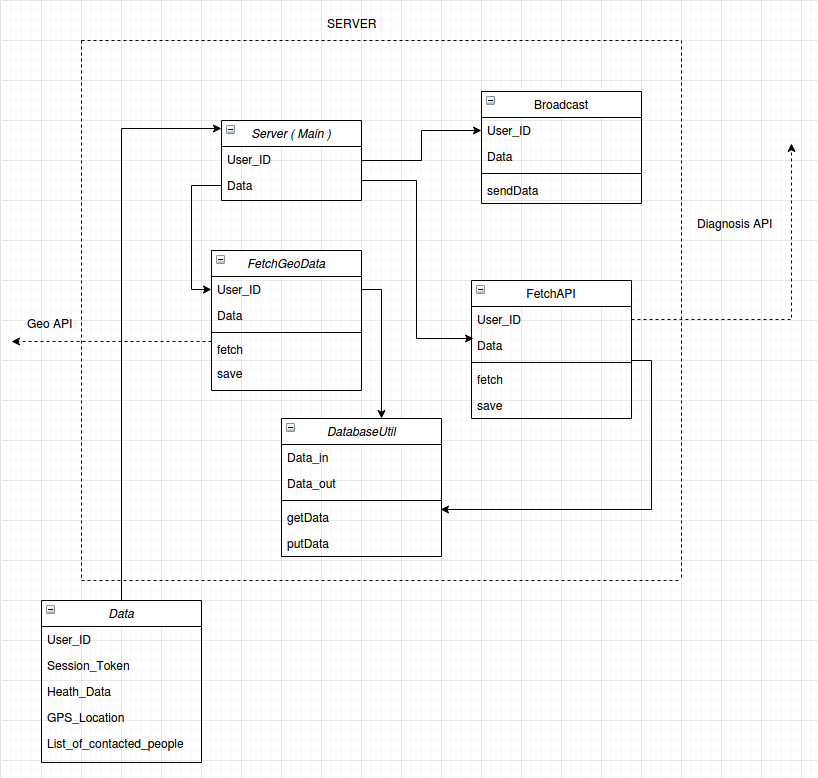
\includegraphics[width=8cm, height=10cm]{UML_Class_Server}
  \caption[Caption for LOF]{Class Diagram of Server\footnotemark}
\end{figure}

\begin{figure}[h!]
  \centering
  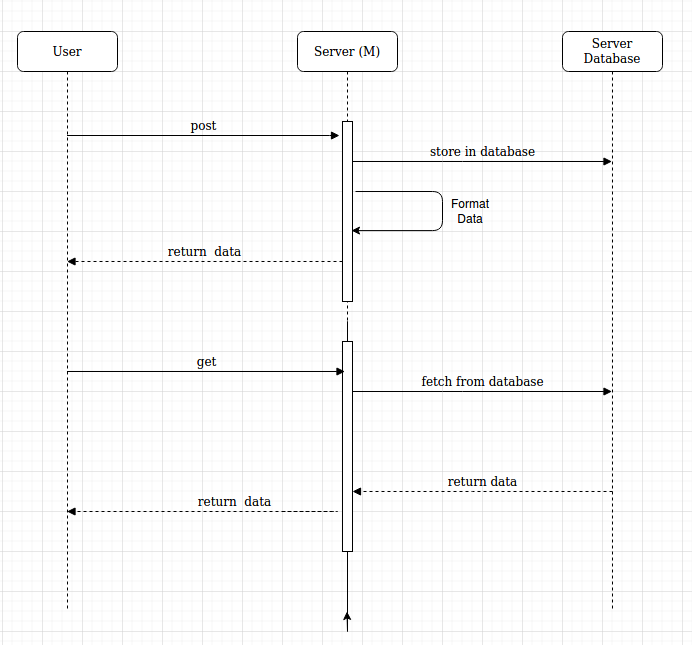
\includegraphics[width=8cm, height=10cm]{UML_Sequence_Server}
  \caption[Caption for LOF]{Sequence Diagram of Server\footnotemark}
\end{figure}

\pagebreak
\subsection{App}

This app keeps the user informed if he/she has been in contact with a covid-19 patient recently. It makes use of Bluetooth to scan for nearby devices using techniques mentioned in the paper~\cite{5}. This ensure safety and reliability. It also find the geographical coordinates and sends it to the server at a timely interval so that exact, precise location can be determined using techniques in ~\cite{3} and ~\cite{4}.\newline
It also consists of an UI, so that the user can type in his symptoms, personal information, etc. which will help in diagnosing the patient using the API mentioned in the literature review section.

\begin{figure}[h!]
  \centering
  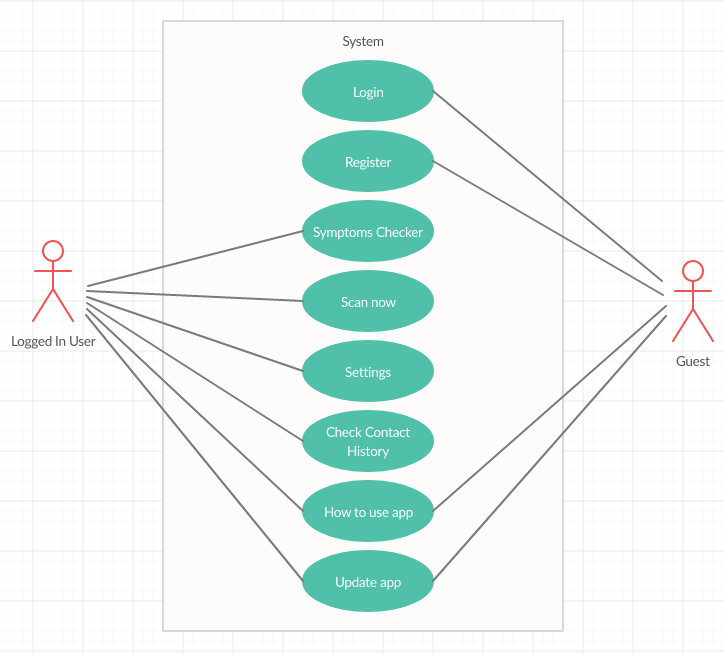
\includegraphics[width=8cm, height=7cm]{UML_UseCase_App}
  \caption[Caption for LOF]{Use Case diagram of App\footnotemark}
\end{figure}

The use cases include:
\begin{enumerate}
  \setlength\itemsep{0.2em}
  \item Login
  \item Register
  \item Symptoms checker
  \item Scan now
  \item Settings
  \item Check contact history
  \item How to use app
  \item Update app
\end{enumerate}
\newline
The different actors that will be using this app are:
\begin{enumerate}
  \item Logged in user
  \item Guest
\end{enumerate}
The use case diagram in Figure 3 shows the use cases an actor can use.
\newline\newline
The entire flow of the app is shown in the Figures 4 and 5.

\begin{figure}[h!]
  \centering
  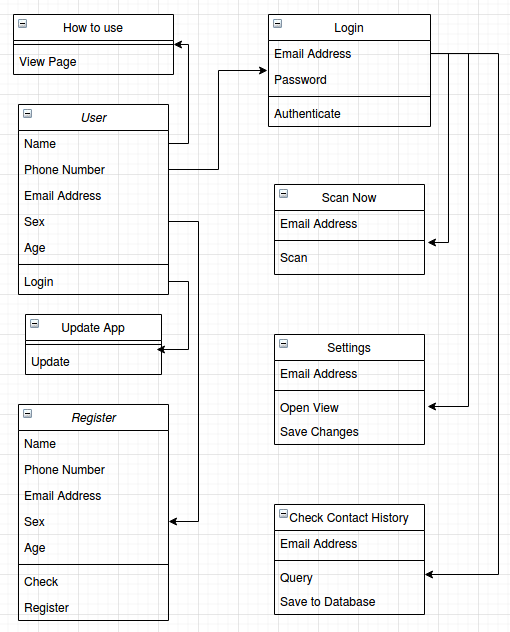
\includegraphics[width=8cm, height=10cm]{UML_Class_App}
  \caption[Caption for LOF]{Class Diagram of App\footnotemark}
\end{figure}

\begin{figure}[h!]
  \centering
  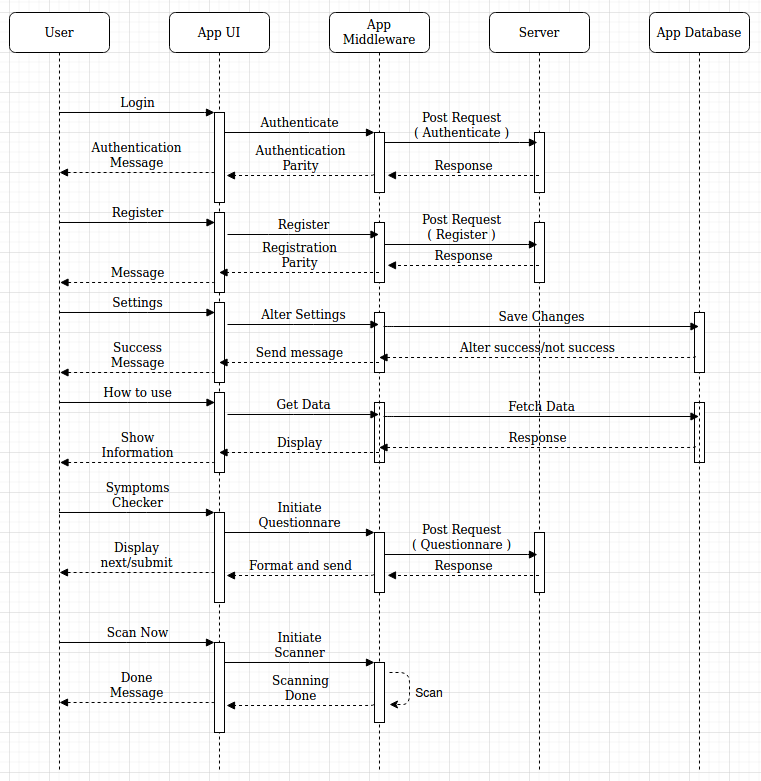
\includegraphics[width=8cm, height=10cm]{UML_Sequence_App}
  \caption[Caption for LOF]{Sequence Diagram of App\footnotemark}
\end{figure}

\newline\newline
The app serves as a tool for the user to get his details uploaded to the cloud and get feedback.
This app helps in regularly monitoring surrounding using Bluetooth and GPS at a optimal fixed interval as given in the papers~\cite{3},~\cite{4} and~\cite{5}.

\subsection{Conclusion and Future Work}
This system along with all the safe, reliable and modern techniques will help reducing the spread of the virus with less work, confusion and panic by a great extent. Timely informing the various subscribers involved will lead to effective healthcare, decision making, etc. A even better system can be implemented by replacing the existing algorithms used, by better ones as time goes by.

{\small
\bibliographystyle{ieee}
\bibliography{egbib}
}

\end{document}